\section{Probability Theory Bounds}\label{sec:bounds}

In this section we present our key insight as a general bound on the expectation of a r.v. and investigate a few special cases which will have applications for bounding rewards in POMDP scenarios.


\subsection{General Bounds}\label{sec:general_bounds}
\begin{figure}[h]
	\centering
	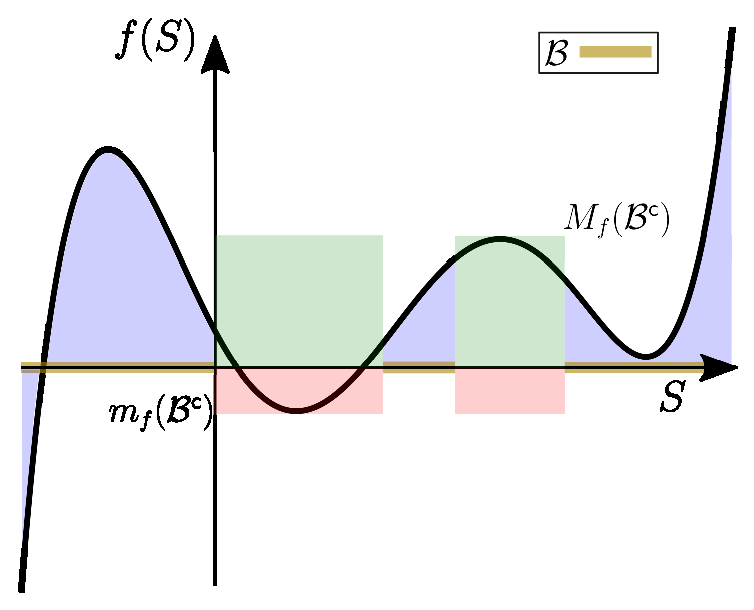
\includegraphics[width=0.4\linewidth]{bounds.eps}
	\caption{The different elements of the bounds of \cref{thm:general_bounds} are seen in the figure. The blue area is preserved as is, and is seen in the bounds as the partial expectation that we explicitly calculate ($\partialexpectation{f(\RV)}{\subSpace}$). The green and red areas are the upper ($M_f(\stcomp{\subSpace})$) and lower ($m_f(\stcomp{\subSpace})$) bounds respectively which need to be weighted by the probability that the variable is found in the compliment subset ($\measure{\stcomp{\subSpace}}$)}
	\label{fig:general_bounds}
\end{figure}
The partial expectation of a r.v. may at times be easier to calculate than the total expectation (the partial expectation is related to but not equivalent to the conditional expectation). We start by introducing the following novel bounds on the difference between the expected value of a given function and its partial expectation.

\begin{theoremE}[][end, no link to proof]
	\label{thm:general_bounds}
	Let $\RV$ be an arbitrary r.v. such that $\variable\in\Space$. Consider an arbitrary function  $f\colon\Space\to\R$. Then for any subset $\subSpace\subseteq\Space$, $\lowerbound\leq\expectation{f(\RV)}{}-\partialexpectation{f(\RV)}{\subSpace}\leq\upperbound$, where:
	\begin{subequations}
	\begin{align}
		\lowerbound & = m_f(\stcomp{\subSpace})\measure{\stcomp{\subSpace}}\;,\label{eq:bound_lower}
		\\
		\upperbound & = M_f(\stcomp{\subSpace})\measure{\stcomp{\subSpace}}\;,
	\end{align}
	\end{subequations}
	and $m_f(\subSpace)$, $M_f(\subSpace)$ are defined as the infimum and supremum of $f$ over the set $\subSpace$ respectively.
\end{theoremE}

\begin{proofE}
	\begin{align*}
		\expectation{f(\RV)}{\RV} & = \expectation{f(\RV)\1{\RV\in \subSpace}}{\RV}+ \expectation{f(\RV)\1{\RV\in \stcomp{\subSpace}}}{\RV}
		\\
		& \leq \expectation{f(\RV)\1{\RV\in \subSpace}}{\RV} +M_f(\stcomp{\subSpace})\expectation{\1{\RV\in \stcomp{\subSpace}}}{\RV}
		\\
		& =\expectation{f(\RV)\1{\RV\in \subSpace}}{\RV} +M_f(\stcomp{\subSpace})\measure{\stcomp{\subSpace}}
		\\
		& =\partialexpectation{f(\RV)}{\subSpace} +M_f(\stcomp{\subSpace})\measure{\stcomp{\subSpace}}\qed
	\end{align*}
\end{proofE}

\begin{theoremE}[][end, no link to proof]
	\label{thm:general_bounds_multi}
	Let $\RV$ be an arbitrary r.v. such that $\variable\in\Space$, and  $f\colon\Space\to\R$ be some function. Then for any subset $\subSpace\subseteq\Space$, $\lowerbound\leq\expectation{f(\RV)}{}-\partialexpectation{f(\RV)}{\subSpace}\leq\upperbound$, where:
	\begin{subequations}
		\begin{align}
			\lowerbound & = \sum_{i=1}^Nm_f(\stcompI{\subSpace}{i})\measure{\stcompI{\subSpace}{i}}\;,
			\\
			\upperbound & = \sum_{i=1}^NM_f(\stcompI{\subSpace}{i})\measure{\stcompI{\subSpace}{i}}\;,
		\end{align}
	\end{subequations}
	and $\bigcup\limits_i^N\stcompI{\subSpace}{i}=\stcomp{\subSpace}$, $\stcompI{\subSpace}{i}\cap\stcomp{\subSpace}_j=\emptyset$.
\end{theoremE}
\begin{proofE}
	The proof is similar to that of \cref{thm:general_bounds}, but with an extra step,
	\begin{align*}
		\expectation{f(\RV)}{\RV} & = \expectation{f(\RV)\1{\RV\in \subSpace}}{\RV}+ \expectation{f(\RV)\1{\RV\in \stcomp{\subSpace}}}{\RV}
		\\&=\expectation{f(\RV)\1{\RV\in \subSpace}}{\RV}+\sum_{i=1}^N\expectation{f(\RV)\1{\RV\in \stcompI{\subSpace}{i}}}{\RV}\\
		&\leq\partialexpectation{f(\RV)}{\subSpace} +\sum_{i=1}^NM_f(\stcompI{\subSpace}{i})\measure{\stcompI{\subSpace}{i}}\qed
	\end{align*}
\end{proofE}

For clarity we also provide the following definitions:
\begin{align*}
		\measure{\subSpace} & \triangleq \expectation{\1{\RV\in \subSpace}}{},\\
		\partialexpectation{f(\RV)}{\subSpace} &\equiv\expectation{f\left(\RV\right)\mid\RV\in\subSpace}{}\measure{\subSpace}.
\end{align*}

All proofs can be found in the \nameref{sec:appendix} and are given only on the upper bound when the lower bound can be reached in a similar manner. A more generalized version of \cref{thm:general_bounds} is also given in supplementary material.
Without loss of generality $\measure{\stcomp{\subSpace}}$ and $1-\measure{\subSpace}$ will be used interchangeably depending on the need, where the use of $1-\measure{\subSpace}$ will often be preferred due to computational benefits.


\Cref{fig:general_bounds} illustrates how we change part of the function in order to bound the expectation in an adaptive fashion. To the best of our knowledge, the bounds given in \cref{thm:general_bounds} are novel and have not previously appeared in the literature.

From inequality \eqref{eq:bound_lower}, if we assume $f(\variable)\geq0$, then $\partialexpectation{f(\RV)}{\subSpace}\geq0$ and we arrive at $\expectation{f(\RV)}{}\geq m_f(\stcomp{\subSpace})\prob{\RV\in\stcomp{\subSpace}},$ which is the generalized Markov inequality~\cite{Durrett19book}. In~\cite{Ogasawara21} the authors show an improvement on the Markov inequality by also using partial expectations, although their approach assumes that the function $f(\variable)$ is non-negative strictly increasing; further generalization of the Markov inequality has also been proposed by~\cite{Bhat22spl}.


\subsection{Special cases}
We explore several special cases relevant to planning and computation efficiency. The following examples are but a small subset of the possible applications.

We begin with $\subSpace$ given as a superset of the subset $\subSpace^\prime$ (i.e. $\subSpace^\prime\subseteq\subSpace$), possible motivation for such an extrapolation would arise from the computation advantage in calculating the extreme values of $\stcomp{\subSpace^\prime}$ over $\stcomp{\subSpace}$. The trivial example of setting $\subSpace^\prime=\emptyset$ leads directly to the global extrema, which can be calculated offline when discussing online algorithms.
\begin{propositionE}[][end, no link to proof]
	\label{thm:bound_diff}
	Consider a r.v. $\RV$ and a function $f$ as defined in \cref{thm:general_bounds}. Let us define the subsets $\subSpace$ and $\subSpace^\prime$ such that $\subSpace^\prime\subseteq\subSpace\subseteq\Space$. Then $\lowerbound\leq\expectation{f(\RV)}{}-\partialexpectation{f(\RV)}{\subSpace}\leq\upperbound$, where:
	\begin{subequations}
		\begin{align}
			\lowerbound & = m_f(\stcomp{\subSpace^\prime})\measure{\stcomp{\subSpace}}\;,
			\\
			\upperbound & = M_f(\stcomp{\subSpace^\prime})\measure{\stcomp{\subSpace}}\;.
		\end{align}
	\end{subequations}
\end{propositionE}
\begin{proofE}
	From \cref{thm:general_bounds} we have
	\begin{align*}
		\expectation{f(\RV)}{\RV} & \leq\partialexpectation{f(\RV)}{\subSpace} +M_f(\stcomp{\subSpace})\measure{\stcomp{\subSpace}}
		\intertext{Given that $\subSpace^\prime\subseteq\subSpace$, then $\stcomp{\subSpace}\subseteq\stcomp{\subSpace^\prime}$\;, leading directly to $M_f(\stcomp{\subSpace})\leq M_f(\stcomp{\subSpace^\prime})$, thus}
		& \leq\partialexpectation{f(\RV)}{\subSpace} +M_f(\stcomp{\subSpace^\prime})\measure{\stcomp{\subSpace}}\qed
	\end{align*}
\end{proofE}

In \cref{thm:general_bounds} the subset defines the minimum and maximum. Alternatively, one could define the subset via the minimum and maximum. (For further motivation see \cref{sec:complexity}.)

\begin{propositionE}[][end, no link to proof]
	\label{thm:bound_epsilon}
	Consider a r.v. $\RV$ and a function $f$ as defined in \cref{thm:general_bounds}. Let $\subSpace$ be a subset defined as $\subSpace\triangleq\{\variable\in\Space \mid f\left(\variable\right) < \varepsilon\lor f\left(\variable\right) > \varepsilon^\prime\}$ then $\exists\varepsilon,\varepsilon^\prime$ such that $\varepsilon\leq\varepsilon^\prime$ and $\lowerbound\leq\expectation{f(\RV)}{}-\partialexpectation{f(\RV)}{\subSpace}\leq\upperbound$, where:
	\begin{subequations}
		\begin{align}
			\lowerbound & =\varepsilon\measure{\stcomp{\subSpace}}\;,
			\\
			\upperbound & =\varepsilon^\prime\measure{\stcomp{\subSpace}}\;.
		\end{align}
	\end{subequations}
\end{propositionE}
\begin{proofE}
	By definition of $\subSpace$, $M_f(\stcomp{\subSpace})\leq\varepsilon^\prime$,  thus
	\begin{equation*}
		\expectation{f(\RV)}{\RV}\leq\partialexpectation{f(\RV)}{\subSpace} +\varepsilon^\prime\measure{\stcomp{\subSpace}}\qed
	\end{equation*}
\end{proofE}

In the following propositions we will look into bounding the expectation of two r.v.s under various assumptions. We start by simply bounding the joint expectation,

\begin{propositionE}[][end, no link to proof]
	\label{thm:bound_multi_cond}
	Consider two arbitrary r.v.s $\RV$ and $\RVI$ such that $\variable\in\Space$ and $\variableI\in\SpaceI$. Let $f\colon\left(\Space,\SpaceI\right)\to\R$ be some arbitrary function, let $\subSpaceI{\variable}$ be an arbitrary subset of $\Space$ and let $\subSpaceI{\variableI}(\variable)$ be an arbitrary subset of $\SpaceI$ as a function of $\variable$. Then $\lowerbound\leq\expectation{f(\RV,\RVI)}{\RV,\RVI}-\partialexpectation{\partialexpectation{f(\RV,\RVI)}{\subSpaceI{\variableI}(\RV)}}{\subSpaceI{\variable}}\leq\upperbound$, where:
	\begin{small}
		\begin{subequations}
			\begin{align}
				\begin{split}
					\lowerbound & = \partialexpectation{m_f(\RV,\stcompI{\subSpace}{\variableI}(\RV))\measure{\stcompI{\subSpace}{\variableI}(\RV)}}{\subSpaceI{\variable}}
					\\
					& \phantomeq+\measure{\stcompI{\subSpace}{\variable}}\left(\inf_{\variable\in\stcompI{\subSpace}{\variable}}\partialexpectation{f(\variable,\RVI)}{\subSpaceI{\variableI}(\variable)}+\inf_{\variable\in\stcompI{\subSpace}{\variable}}\left\{\measure{\stcompI{\subSpace}{\variableI}(\variable)}m_f\left(\variable,\stcompI{\subSpace}{\variableI}(\variable)\right)\right\}\right)\;,
				\end{split}
				\\
				\begin{split}
					\upperbound & = \partialexpectation{M_f(\RV,\stcompI{\subSpace}{\variableI}(\RV))\measure{\stcompI{\subSpace}{\variableI}(\RV)}}{\subSpaceI{\variable}}
					\\
					& \phantomeq+\measure{\stcompI{\subSpace}{\variable}}\left(\sup_{\variable\in\stcompI{\subSpace}{\variable}}\partialexpectation{f(\variable,\RVI)}{\subSpaceI{\variableI}(\variable)}+\sup_{\variable\in\stcompI{\subSpace}{\variable}}\left\{\measure{\stcompI{\subSpace}{\variableI}(\variable)}M_f\left(\variable,\stcompI{\subSpace}{\variableI}(\variable)\right)\right\}\right)\;,
				\end{split}
			\end{align}
		\end{subequations}
	\end{small}
	and $m_f(\subSpaceI{\variable},\RVI)\triangleq\inf\limits_{\variable\in\subSpaceI{\variable}}f(\variable,\RVI)$, $M_f(\subSpaceI{\variable},\RVI)\triangleq\sup\limits_{\variable\in\subSpaceI{\variable}}f(\variable,\RVI)$.
\end{propositionE}
\begin{proofE}
	We begin by applying \cref{thm:general_bounds} to the inner expectation
	\begin{align*}
		\expectation{\expectation{f(\RV,\RVI)}{\RVI\mid\RV}}{\RV} & \leq \E_{\RV}\Bigl[\partialexpectation{f(\RV,\RVI)}{\subSpaceI{\variableI}(\RV)}+M_f(\RV,\stcomp{\subSpaceI{\variableI}(\RV)})\measure{\stcomp{\subSpaceI{\variableI}(\RV)}}\Bigr]\\
		\intertext{Now applying \cref{thm:general_bounds} to the outer expectation}
		\begin{split}
			&\leq\partialexpectation{\partialexpectation{f(\RV,\RVI)}{\subSpaceI{\variableI}(\RV)}}{\subSpaceI{\variable}}
			+\partialexpectation{M_f(\RV,\stcompI{\subSpace}{\variableI}(\RV))\measure{\stcompI{\subSpace}{\variableI}(\RV)}}{\subSpaceI{\variable}}
			\\
			& \phantomeq+\measure{\stcompI{\subSpace}{\variable}}\sup_{\variable\in\stcompI{\subSpace}{\variable}}\partialexpectation{f(\variable,\RVI)}{\subSpaceI{\variableI}(\variable)}\\
			&\phantomeq
			+\measure{\stcompI{\subSpace}{\variable}}\sup_{\variable\in\stcompI{\subSpace}{\variable}}\left\{\measure{\stcompI{\subSpace}{\variableI}(\variable)}M_f\left(\variable,\stcompI{\subSpace}{\variableI}(\variable)\right)\right\}\qed
		\end{split}
	\end{align*}
\end{proofE}

\begin{figure*} [h]
	\centering
	\begin{subfigure}[t]{0.45\textwidth}
		\centering
		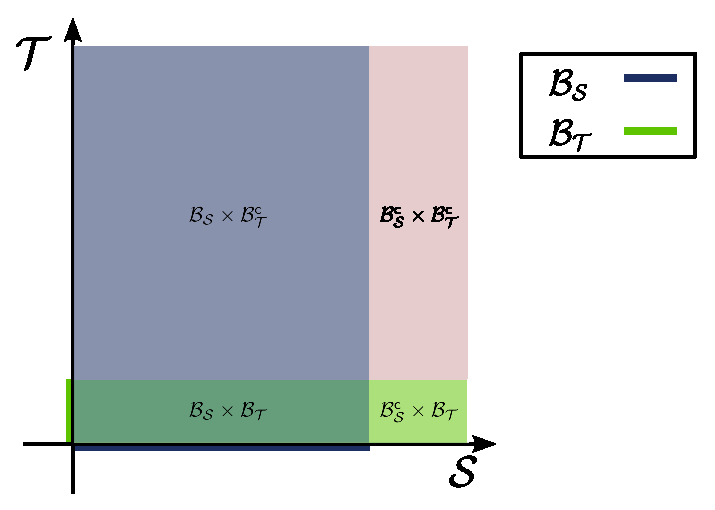
\includegraphics[width= 0.95\linewidth,clip]{independent_sets.eps}
		\caption{Visualization of the partitioning dictated by \cref{thm:bound_multi_ind_2}. We can explicitly factor the joint domain $\subSpace$ into the Cartesian product $\subSpaceI{\variable}\times\subSpaceI{\variableI}$, thus in this scenario $\stcomp{\subSpace}=\left(\subSpaceI{\variable}\times\stcompI{\subSpace}{\variableI}\right)\cup\left(\stcompI{\subSpace}{\variable}\times\subSpaceI{\variableI}\right)\cup\left(\stcompI{\subSpace}{\variable}\times\stcompI{\subSpace}{\variableI}\right)$}
		\label{fig:ind_sets}
	\end{subfigure}
	\hfill
	\begin{subfigure}[t]{0.45\textwidth}
		\centering
		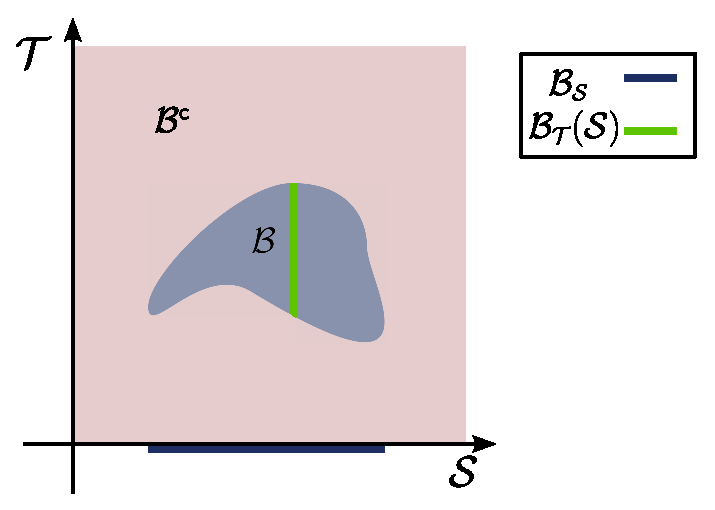
\includegraphics[width= 0.95\linewidth,clip]{dependent_sets.eps}
		\caption{Visualization of the partitioning dictated by \cref{thm:bound_multi}. The set $\subSpace$ is a general subset of the joint sample space $(\Space\times\SpaceI)$, as such it cannot necessarily be represented as a Cartesian product of two independent sets}
		\label{fig:dep_sets}
	\end{subfigure}
	\caption{Joint domain partitioning employed in the different scenarios}
	\label{fig:sets}
\end{figure*}


\begin{propositionE}[][end, no link to proof]
	\label{thm:bound_multi_ind}
	Consider two arbitrary independent r.v.s $\RV$ and $\RVI$ such that $\variable\in\Space$ and $\variableI\in\SpaceI$. Let $f\colon\left(\Space,\SpaceI\right)\to\R$ be some arbitrary function and let $\subSpaceI{\variable}$ and $\subSpaceI{\variableI}$ be arbitrary subsets of $\Space$ and $\SpaceI$ respectively. Then $\lowerbound\leq\expectation{f(\RV,\RVI)}{\RV,\RVI}-\partialexpectation{\partialexpectation{f(\RV,\RVI)}{\subSpaceI{\variableI}}}{\subSpaceI{\variable}}\leq\upperbound$, where:
	\begin{subequations}
		\begin{align}
			\begin{split}
				\lowerbound & = \measure{\stcompI{\subSpace}{\variableI}}\partialexpectation{m_f(\RV,\stcompI{\subSpace}{\variableI})}{\subSpaceI{\variable}}
				+\measure{\stcompI{\subSpace}{\variable}}\inf_{\variable\in\stcompI{\subSpace}{\variable}}\partialexpectation{f(\variable,\RVI)}{\subSpaceI{\variableI}}\\
				&\phantomeq+\measure{\stcompI{\subSpace}{\variableI}}\measure{\stcompI{\subSpace}{\variable}}m_f\left(\stcompI{\subSpace}{\variable},\stcompI{\subSpace}{\variableI}\right)\;,
			\end{split}
			\\
			\begin{split}
				\upperbound & = \measure{\stcompI{\subSpace}{\variableI}}\partialexpectation{M_f(\RV,\stcompI{\subSpace}{\variableI})}{\subSpaceI{\variable}}
				+\measure{\stcompI{\subSpace}{\variable}}\sup_{\variable\in\stcompI{\subSpace}{\variable}}\partialexpectation{f(\variable,\RVI)}{\subSpaceI{\variableI}}\\
				&\phantomeq+\measure{\stcompI{\subSpace}{\variableI}}\measure{\stcompI{\subSpace}{\variable}}M_f\left(\stcompI{\subSpace}{\variable},\stcompI{\subSpace}{\variableI}\right)\;,
			\end{split}
		\end{align}
	\end{subequations}
	and $\subSpaceI{\variable}(\variableI)=\subSpaceI{\variable}$, $\subSpaceI{\variableI}(\variable)=\subSpaceI{\variableI}$.
\end{propositionE}
\begin{proofE}
	Given that the r.v.s and subsets are independent, \cref{thm:bound_multi_cond} simplifies trivially to the bounds
\end{proofE}

We note that the relation between $\subSpaceI{\variable}$, $\subSpaceI{\variableI}$ and the joint subset ($\subSpace^\prime$) is given by $\subSpace^\prime=\subSpaceI{\variable}\times\subSpaceI{\variableI}$, this does not imply that $\stcomp{\subSpace^\prime}=\stcompI{\subSpace}{\variable}\times\stcompI{\subSpace}{\variableI}$. Furthermore it can be easily shown that the number of terms is exponential with the number of independent variables, thus a simpler bound is desirable. Under the same assumptions, but with further relaxation of the bounds, we can arrive at simplified bounds given by

\begin{propositionE}[][end, no link to proof]
	\label{thm:bound_multi_ind_2}
	Consider two arbitrary independent r.v.s $\RV$ and $\RVI$ and a function $f$ as in \cref{thm:bound_multi_cond}. Let $\subSpaceI{\variable}$ and $\subSpaceI{\variableI}$ be arbitrary subsets of $\Space$ and $\SpaceI$ respectively. Then $\lowerbound\leq\expectation{f(\RV,\RVI)}{\RV,\RVI}-\partialexpectation{\partialexpectation{f(\RV,\RVI)}{\subSpaceI{\variableI}}}{\subSpaceI{\variable}}\leq\upperbound$, where:
	\begin{subequations}
		\begin{align}
			\lowerbound & = \left(1-\measure{\subSpaceI{\variable}}\measure{\subSpaceI{\variableI}}\right)m_f(\stcomp{\subSpace^\prime})\;, \\
			\upperbound & = \left(1-\measure{\subSpaceI{\variable}}\measure{\subSpaceI{\variableI}}\right)M_f(\stcomp{\subSpace^\prime})\;,
		\end{align}
	\end{subequations}
	and $\subSpace^\prime\triangleq\subSpaceI{\variable}\times\subSpaceI{\variableI}$.
\end{propositionE}
\begin{proofE}
	\begin{align*}
		\expectation{f(\RV,\RVI)}{\RV,\RVI}-\partialexpectation{\partialexpectation{f(\RV,\RVI)}{\subSpaceI{\variableI}}}{\subSpaceI{\variable}} & \leq M_f(\stcomp{\subSpace^\prime})\measure{\stcomp{\subSpace^\prime}}                                            \\
		& =M_f(\stcomp{\subSpace^\prime})\left(1-\measure{\subSpaceI{\variable}\times\subSpaceI{\variableI}}\right)         \\
		& =M_f(\stcomp{\subSpace^\prime})\left(1-\measure{\subSpaceI{\variable}}\measure{\subSpaceI{\variableI}}\right)\qed
	\end{align*}
\end{proofE}

Finally, we examine how we can leverage possible knowledge of the structure of $f$ to allow for intuitive bounds on seemingly unbounded functions. We begin by bounding the $\log$ function, a common function in information theoretical rewards.

\begin{propositionE}[][end, no link to proof]
	\label{thm:bound_log}
	Let $\RV$ and $f$ be defined as in \cref{thm:general_bounds} and consider the specific structure of $f(\variable)\triangleq g(\variable)\log h(\variable)$, where $h$ is a non-negative function and let $\subSpace$ be an arbitrary subset. Then $\lowerbound\leq\expectation{f(\RV)}{}-\partialexpectation{f(\RV)}{\subSpace}\leq\upperbound$, where:
	\begin{subequations}
		\begin{align}
			\lowerbound & = \measure{\stcomp{\subSpace}}
			\min\left\{m_g(\stcomp{\subSpace})\log m_h(\stcomp{\subSpace}),M_g(\stcomp{\subSpace})\log m_h(\stcomp{\subSpace})\right\}\;,\label{eq:bound_lower_log}\\
			\upperbound & = \measure{\stcomp{\subSpace}}
			\max\left\{m_g(\stcomp{\subSpace})\log M_h(\stcomp{\subSpace}),M_g(\stcomp{\subSpace})\log M_h(\stcomp{\subSpace})\right\}\;\label{eq:bound_upper_log}.
		\end{align}
	\end{subequations}
\end{propositionE}
\begin{proofE}
	Assuming $g(\variable)\geq 0$
	\begin{equation*}
		M_f(\stcomp{\subSpace})=\max_{\variable\in\stcomp{\subSpace}}\{g(\variable)\log h(\variable)\}\leq\max\left\{
		\begin{aligned}
			& M_g(\stcomp{\subSpace})\log M_h(\stcomp{\subSpace})\;, \\
			& m_g(\stcomp{\subSpace})\log M_h(\stcomp{\subSpace})
		\end{aligned}\right\}\qed
	\end{equation*}
	The assumption of $g(\variable)\geq 0$ can also be easily dropped for a more general bound.
\end{proofE}
Further cases pertaining to bounds with multiple random variables are studied in the \nameref{sec:appendix}.

\begin{propositionE}[][end, no link to proof]
\label{thm:bound_exp}
	Let $\RV\in\R^N$ and $\RVI\in\R^m$ be two r.v.. Let $f$ be of the specific structure $f(\variable)\triangleq \expectation{\log g(\variable,\RVI)}{\RVI\mid\variable}\colon\R^N\to\R$, where $g$ is non-negative. Thus by \cref{thm:general_bounds} the difference $\expectation{\expectation{\log g(\RV,\RVI)}{\RVI\mid\RV}}{\RV}-
	\partialexpectation{\expectation{\log g(\RV,\RVI)}{\RVI\mid\RV}}{\subSpace}$ is bounded above and below by
	\begin{align}
		\begin{split}
			\lowerbound=&\measure{\stcomp{\subSpace}}\log\left(\inf_{\variable\in\stcomp{\subSpace},\variableI}g(\variable,\variableI)\right),
		\end{split}\label{eq:bound_lower_exp}
		\\
		\begin{split}
			\upperbound=&\measure{\stcomp{\subSpace}}\log\left(\sup_{\variable\in\stcomp{\subSpace},\variableI}g(\variable,\variableI)\right).
		\end{split}\label{eq:bound_upper_exp}
	\end{align}
\end{propositionE}
\begin{proofE}
	\begin{align*}
		\expectation{\expectation{\log f(\RV,\RVI)}{\RVI\mid\RV}}{\RV}&=\expectation{\expectation{\log \frac{f(\RV,\RVI)}{\varepsilon(\RVI)}}{\RVI\mid\RV}}{\RV}+\expectation{\expectation{\log \varepsilon(\RVI)}{\RVI\mid\RV}}{\RV}
		\\
		&=\expectation{\expectation{\log \frac{f(\RV,\RVI)}{\varepsilon(\RVI)}}{\RVI\mid\RV}}{\RV}+\expectation{\log \varepsilon(\RVI)}{\RVI}
		\\
		\begin{split}
			&\leq\partialexpectation{\expectation{\log f(\RV,\RVI)}{\RVI\mid\RV}}{\subSpace}-\partialexpectation{\expectation{\log \varepsilon(\RVI)}{\RVI\mid\RV}}{\subSpace}\\
			&\phantomeq+\left(1-\measure{\subSpace}\right)\log\max_{\variableI}\varepsilon(\variableI)+\expectation{\log \varepsilon(\RVI)}{\RVI}\qedhere
		\end{split}
	\end{align*}
\end{proofE}

\subsection{Bound Properties}
The bounds from \cref{thm:general_bounds} have several desirable properties for bound based decision making algorithms, the principle of which is incrementality, allowing for the tightening of the bounds while reusing parts of the original bounds.


\begin{corollaryE}[Incrementality][end, no link to proof]
	\label{thm:incrementality}
	Given a subset $\subSpace^\prime$ such that $\subSpace\subseteq\subSpace^\prime$ the bounds as defined in \cref{thm:general_bounds} can be calculated incrementally for $\subSpace^\prime$.  In other words, calculations only within the new subset $\subSpace_{\textrm{\textup{new}}}\triangleq\subSpace^\prime\setminus\subSpace$ are needed. This can be expressed explicitly as follows:
	\begin{align}
		\partialexpectation{f(\RV)}{\subSpace^\prime} & =\partialexpectation{f(\RV)}{\subSpace}+\partialexpectation{f(\RV)}{\subSpace_{\textrm{\textup{new}}}}\;,
		\\
		\measure{\subSpace^\prime}& =\measure{\subSpace}+\measure{\subSpace_{\textrm{\textup{new}}}}\;.
	\end{align}
	The infimum and supremum are partially incremental, depending on the scenario as described below
	\begin{subequations}
		\begin{align}
			m_f(\stcomp{\subSpace^\prime})
			& =\begin{cases}
				m_f(\stcomp{\subSpace}) & \textup{if}\ m_f(\stcomp{\subSpace})<m_f(\subSpace_{\textrm{\textup{new}}}) \\
				\textup{by definition}  & \textup{else}
			\end{cases}\;, \\
			M_f(\stcomp{\subSpace^\prime})
			& =\begin{cases}
				M_f(\stcomp{\subSpace}) & \textup{if}\ M_f(\stcomp{\subSpace})>M_f(\subSpace_{\textrm{\textup{new}}}) \\
				\textup{by definition}  & \textup{else}
			\end{cases}\;.
		\end{align}
	\end{subequations}
\end{corollaryE}
\begin{proofE}
	\begin{align*}
		\partialexpectation{f(\RV)}{\subSpace^\prime} & =\expectation{f(\RV)\1{\RV\in\subSpace^\prime}}{}\\
		& =\expectation{f(\RV)\left(\1{\RV\in\subSpace}+\1{\RV\in\subSpace_{\textrm{\textup{new}}}}\right)}{}\\
		& =\partialexpectation{f(\RV)}{\subSpace}+\partialexpectation{f(\RV)}{\subSpace_{\textrm{\textup{new}}}}
	\end{align*}
	The proof for $\measure{\subSpace^\prime}$ follows the same logic.

	$\stcomp{\subSpace}=\subSpace_{\textrm{\textup{new}}}\cup\stcomp{\subSpace^\prime}$, thus $M_f(\stcomp{\subSpace})=\max\{M_f(\subSpace_{\textrm{\textup{new}}}),M_f(\stcomp{\subSpace^\prime})\}$, if $M_f(\stcomp{\subSpace})>M_f(\subSpace_{\textrm{\textup{new}}})$, then implicitly $M_f(\stcomp{\subSpace})\neq M_f(\subSpace_{\textrm{\textup{new}}})$ leaving us with $M_f(\stcomp{\subSpace})=M_f(\stcomp{\subSpace^\prime})$. If $M_f(\stcomp{\subSpace})=M_f(\subSpace_{\textrm{\textup{new}}})$ then we gain no information on $M_f(\stcomp{\subSpace^\prime})$, leaving us with $M_f(\stcomp{\subSpace})\geq M_f(\stcomp{\subSpace^\prime})$.
\end{proofE}


\begin{corollaryE}[Convergence][end, no link to proof]
	\label{thm:convergence}
	The bounds as defined in \cref{thm:general_bounds} converge to zero with respect to the set $\subSpace$, meaning the partial expectation converges to the true expectation when $\subSpace=\Space$.
\end{corollaryE}
\begin{proofE}
	By definition $\measure{\Space}=1$ and $\partialexpectation{f(\RV)}{\Space}=\expectation{f(\RV)}{\RV}$, thus we immediately arrive at $\lowerbound(\Space)=\upperbound(\Space)=0$
\end{proofE}

\begin{corollaryE}[Monotonicity][end, no link to proof]
	\label{thm:monotonicity}
	The bounds as defined in \cref{thm:general_bounds} are monotonic with respect to the subspace. Specifically:
	\begin{subequations}
		\begin{align}
			\lowerbound(\subSpace) & \leq\lowerbound(\subSpace^\prime)\;, \\
			\upperbound(\subSpace) & \geq\upperbound(\subSpace^\prime)\;,
		\end{align}
	\end{subequations}
	for $\subSpace\subseteq\subSpace^\prime$. Moreover these bounds are strictly monotonic when $\subSpace_{\textrm{\textup{new}}}$ is measurable (i.e. $\measure{\subSpace_{\textrm{\textup{new}}}}\neq0$).
\end{corollaryE}
\begin{proofE}
	Let us define $\subSpace^\prime\supseteq\subSpace$, thus $M_f(\stcomp{\subSpace^\prime})\leq M_f(\stcomp{\subSpace})$, by \cref{thm:incrementality} we find that $\measure{\subSpace}\leq\measure{\subSpace^\prime}$ thus
	\begin{equation*}
		M_f(\stcomp{\subSpace^\prime})\left(1-\measure{\subSpace^\prime}\right) \leq M_f(\stcomp{\subSpace})\left(1-\measure{\subSpace}\right)\qed
	\end{equation*}
\end{proofE}

\subsection{Complexity}\label{sec:complexity}
Let us denote the complexity of a single evaluation of the function $f$ by $O(\abs{f})$, and the complexity of finding bounds on the infimum and supremum of $f$ by $O(\abs{m})$ and $O(\abs{M})$ respectively. Then the complexity of calculating the bounds in \cref{thm:general_bounds} is given by the complexity of the partial expectation over the set $\subSpace$ and the complexity of finding the infimum and supremum over the set $\stcomp{\subSpace}$, $O\left(\abs{f}\cdot\abs{\subSpace}+\left(\abs{m}+\abs{M}\right)\cdot\abs{\stcomp{\subSpace}}\right)$. When $O(\abs{m}+\abs{M})\ll O(\abs{f})$ then computational savings of approximately $O(\abs{f}\cdot\abs{\stcomp{\subSpace}})$ are attained.

The above assumes that the complexity of division into subsets is trivial. But alternatively, one could select subsets defined by their infimum and supremum as in \cref{thm:bound_epsilon}, thus $O(\abs{m})=O(\abs{M})=O(1)$, but the complexity is simply transferred into finding which elements belong in each subset, this is the case with the Markov inequality. The choice between these two scenarios is per use case.

\subsection{Estimators and Novel Probabilistic Bounds}
An estimator $\hat{P}(\states{})$ of the distribution $\prob{\states{}}$ is given by: $\sum\limits_{i=1}^{N}w^i\delta\left(\states{}-\states{}^i\right)$, where $(\weight{}{i},\states{}^i)$ is a weighted particle sampled from $\prob{\states{}}$. Thus by defining $\estimator{\cdot}{\statesRV{}\sim \prob{\states{}}} \triangleq \expectation{\cdot}{\statesRV{}\sim \hat{P}(\states{})}$, we find $\estimator{g(\states{})}{\statesRV{}}=\int\sum_{i=1}^{N}\weight{}{i}\delta\left(\states{}-\states{}^i\right)g(\states{})\D\states{}=\sum_{i=1}^{N}\weight{}{i}g(\states{}^i),$
which is in practice the expectation with respect to a discrete variable with $\hat{P}\left(\states{}^i\right)=\weight{}{i}$. Thus \cref{thm:general_bounds}, with no additional changes, is also valid for estimators, where the sample space is defined by the set of samples. This also holds true for functions of the pdf, both of the form $\estimator{f(\hat{P}(\states{}))}{}$ and $\estimator{f(\prob{\states{}})}{}$ with appropriate attention given to constructing the bound itself.

When the pdf itself is also estimated as in the case of $\hat{P}(\states{})$, then bounds on the estimated weights may be useful for \cref{thm:general_bounds}, thus we provide \cref{thm:estimator_bound}.

\begin{corollaryE}[][end, no link to proof]
	\label{thm:estimator_bound}
	Let $\{(\weight{}{i},\variable^i)\}^N_{i=1}$ be a set of normalized particles sampled from the distribution $\prob{\variable}$. Then the weights ($\weight{}{i}$) are bounded below and above by
	\begin{subequations}
		\begin{align}
			\lowerbound & =1-\frac{\max \prob{\variable}}{\frac{\min \prob{\variable}}{N-1}+\max\prob{\variable}}\;, \\
			\upperbound & =1-\frac{\min \prob{\variable}}{\frac{\max \prob{\variable}}{N-1}+\min\prob{\variable}}\;.
		\end{align}
	\end{subequations}
\end{corollaryE}
\begin{proofE}
	\begin{align*}
		\min_i \weight{}{i} & =\min_i \frac{\prob{\variable^i}}{\sum_{i=1}^N\prob{\variable^i}}
		\intertext{Let us denote, without loss of generality, $\min\limits_i \prob{\variable^i}$ as $\prob{\variable^1}$, thus}
		& =\frac{\prob{\variable^1}}{\prob{\variable^1}+\sum_{i=2}^N\prob{\variable^i}}          \\
		& \geq\frac{\prob{\variable^1}}{\prob{\variable^1}+(N-1)\max\limits_i\prob{\variable^i}} \\
		& \geq\frac{\min\prob{\variable}}{\min\prob{\variable}+(N-1)\max\prob{\variable}}\qed
	\end{align*}
\end{proofE}

The use of estimators in the field of robotics is often present when we use Monte-Carlo methods for reasoning about future actions. As we are working with estimators, we are interested in how close the estimator is to the theoretical expectation. Via Hoeffding's inequality we arrive at two main claims of our paper; the first is a probabilistic bound between the true expectation and the estimated partial expectation.

\begin{theoremE}[][end, no link to proof]
	\label{thm:partial_hoeffding}
	Consider the set of samples $\{\variable^i\}_{i=1}^N$ drawn from $\RV$, then
	\begin{align*}
		\prob{\lowerbound\leq\expectation{f(\RV)}{}-\partialestimator{f(\RV)}{\subSpace_n}\leq\upperbound}\geq1-\delta&&\forall\delta\in(0,1)\;,
	\end{align*}
	where $\subSpace_n\triangleq\{\variable^i\}_{i=1}^n$ for $n\leq N$,
	\begin{subequations}
		\begin{align}
			\lowerbound & =-\sqrt{\frac{\Delta_f^2}{2N}\log\frac{2}{\delta}}+m_f(\stcomp{\subSpace_n})\estimatedmeasure{\stcomp{\subSpace_n}}\;, \\
			\upperbound & =\sqrt{\frac{\Delta_f^2}{2N}\log\frac{2}{\delta}}+M_f(\stcomp{\subSpace_n})\estimatedmeasure{\stcomp{\subSpace_n}}\;,
		\end{align}
	\end{subequations}
	and $\Delta_f(\subSpace)\triangleq M_f(\subSpace)-m_f(\subSpace)$
\end{theoremE}
\begin{proofE}
	From Hoeffding's inequality on the r.v. $f(\RV)$ the following holds
	\begin{equation*}
		\prob{\abs{\expectation{f(\RV)}{}-\estimator{f(\RV)}{}}\leq t}\geq1-\delta,
	\end{equation*}
	where $t=\sqrt{\frac{\Delta_f^2}{2N}\log\frac{2}{\delta}}$. From the absolute value we have two inequalities, we fill focus on the upper bound.
	With the addition of inequality \refeq{eq:bound_upper} for some subset $\subSpace_n$ of the samples
	\begin{align*}
		& \expectation{f(\RV)}{}-\estimator{f(\RV)}{}+\estimator{f(\RV)}{}-\partialestimator{f(\RV)}{\subSpace}\leq t+M_f(\stcomp{\subSpace})\estimatedmeasure{\stcomp{\subSpace}}, \\
		& \expectation{f(\RV)}{}-\partialestimator{f(\RV)}{\subSpace}\leq t+M_f(\stcomp{\subSpace})\estimatedmeasure{\stcomp{\subSpace}}.
	\end{align*}
	Repeating the procedure for the lower bounds results in the complete bounds.
\end{proofE}

It can be shown that when comparing \cref{thm:partial_hoeffding} to the case of simply taking a Hoeffding bound with $n$ samples from the original distribution, our bounds are tighter when the following inequality is satisfied:
\begin{equation}
	C\cdot\left(\sqrt{\frac{1}{n}}-\sqrt{\frac{1}{N}}\right)\geq\Delta_f(\stcomp{\subSpace_n})\estimatedmeasure{\stcomp{\subSpace_n}}\;,
\end{equation}
where $C\triangleq \Delta_f\sqrt{2\log\frac{2}{\delta}}$. The bound is relevant when $N$ samples are drawn, but evaluation of the function $f$ for all $N$ samples is undesirable, allowing for a controlled way to remove some samples.

The second of the claims is a probabilistic bound between the true expectation and the estimated conditional expectation.
\begin{theoremE}[][end, no link to proof]
	\label{thm:conditional_hoeffding}
	Let $\RV$ be some r.v. and let $\subSpace\subseteq\Space$ be some sample space. Consider the set of samples $\{\variable^i\}_{i=1}^N$ drawn from $\RV\1{\RV\in\subSpace}$, then
	\begin{align*}
		\prob{\lowerbound\leq\expectation{f(\RV)}{}-\measure{\subSpace}\condestimator{f(\RV)}{\subSpace}{}\leq\upperbound}\geq1-\delta&&\forall\delta\in(0,1)\;,
	\end{align*}
	where
	\begin{subequations}
		\begin{align}
			\lowerbound & =-\measure{\subSpace}\sqrt{\frac{\Delta_f(\subSpace)^2}{2N}\log\frac{2}{\delta}}+m_f(\stcomp{\subSpace})\measure{\stcomp{\subSpace}}\;, \\
			\upperbound & =\measure{\subSpace}\sqrt{\frac{\Delta_f(\subSpace)^2}{2N}\log\frac{2}{\delta}}+M_f(\stcomp{\subSpace})\measure{\stcomp{\subSpace}}\;.
		\end{align}
	\end{subequations}
\end{theoremE}
\begin{proofE}
	From Hoeffding's inequality on the r.v. $f(\RV)$ the following holds
	\begin{equation*}
		\prob{\abs{\condexpectation{f(\RV)}{\subSpace}{}-\condestimator{f(\RV)}{\subSpace}{}}\leq t}\geq1-\delta\;,
	\end{equation*}
	where $t=\sqrt{\frac{\Delta_f^2}{2N}\log\frac{2}{\delta}}$. From the absolute value we have two inequalities, we fill focus on the upper bound.
	Multiplying though by $\measure{\subSpace}$ and the addition of inequality \refeq{eq:bound_upper} we find
	\begin{align*}
		& \partialexpectation{f(\RV)}{\subSpace}-\measure{\subSpace}\condestimator{f(\RV)}{\subSpace}{}\leq \measure{\subSpace}t\;,\\
		\begin{split}
			& \expectation{f(\RV)}{}-\partialexpectation{f(\RV)}{\subSpace}+\partialexpectation{f(\RV)}{\subSpace}-\measure{\subSpace}\condestimator{f(\RV)}{\subSpace}{} \\
			& \leq \measure{\subSpace}t+M_f(\stcomp{\subSpace})\measure{\stcomp{\subSpace}}\;,
		\end{split} \\
		& \expectation{f(\RV)}{}-\measure{\subSpace}\condestimator{f(\RV)}{\subSpace}{}\leq\measure{\subSpace}t+M_f(\stcomp{\subSpace})\measure{\stcomp{\subSpace}}\;.
	\end{align*}
\end{proofE}

\noindent Similarly to \cref{thm:partial_hoeffding}, \cref{thm:conditional_hoeffding} offers tighter bounds in comparison to the vanilla Hoeffding bound under the following inequality constraint:
\begin{equation}
	C\cdot\left(\Delta_f-\measure{\subSpace}\Delta_f(\subSpace)\right)\geq \measure{\stcomp{\subSpace}}\Delta_f(\stcomp{\subSpace})\;,
\end{equation}
where $C\triangleq\sqrt{\frac{2}{N}\log\frac{2}{\delta}}$.

Utilizing this bound is relevant when one would like to focus the sampling procedure on a specific area of the distribution, or if only a proposal distribution is available on part of the support, while still being able to make a claim on the expectation. It may be desirable to apply another Hoeffding inequality in order to estimate and bound with the use of $\estimatedmeasure{\subSpace}$.

%We can bound the expectation of $f(\RV)$ by sampling via importance sampling only from the subspace $\subSpace$ via some proposal distribution $q(\variable)$, where the sample space $\subSpace$ is such that $\int_\subSpace q(\variable)\D\variable=1$. This extension of the standard Hoeffding inequality incorporates the use of \cref{thm:general_bounds}, allowing for concentration inequality on the expected value with respect to a partial estimator, and not the complete estimator as is traditionally done.
%
%We will address one special case where $q(\variable)\triangleq \frac{p(\variable)\1{\variable\in\subSpace}}{\int_\subSpace p(\variable)\D\variable}=\frac{p(\variable)\1{\variable\in\subSpace}}{\measure{\subSpace}}$. Under these conditions
%\begin{equation}
%	\partialexpectation{f(\RV)}{\subSpace}\equiv\measure{\subSpace}\expectation{f\left(\RV\right)}{\RV\sim q},
%\end{equation}
%and the bounds of \cref{thm:partial_hoeffding} still hold with probability $\left((1-\delta)(1-\delta^\prime)\right)^2$ for the difference $\expectation{f(\RV)}{\RV\sim p}-
%\measure{\subSpace}\estimator{f\left(\RV\right)}{\RV\sim q}$. Although it might prove necessary to estimate $\measure{\subSpace}$ and apply an additional use of the Hoeffding's inequality.